\begin{center}
	\begin{tabular}{rp{6cm}lp{10cm}}%{rl}
		% after \\: \hline or \cline{col1-col2} \cline{col3-col4} ...
		论文地址:& \href{https://arxiv.org/abs/2010.06253}{https://arxiv.org/abs/2010.06253} \\
		%源码地址:& \href{https://github.com/mocherson/Exp_GNN}{ExpGNN} \\
		关键词:& \textbf{Document Summarization, GAT, BERT} \\
		写于:& \date{2020-10-15}
	\end{tabular}
\end{center}
该论文\cite{cui2020enhancing}针对抽取式文本摘要问题提出了一个基于GNN的方法。现有的抽取式的文档摘要算法中,是通过从文档中抽取一个句子序列作为文档的摘要,但是通常没有考虑句子之间的关系,论文针对这个问题,提出了Topic-GraphSum模型。
\begin{figure}[h]
	\centering
	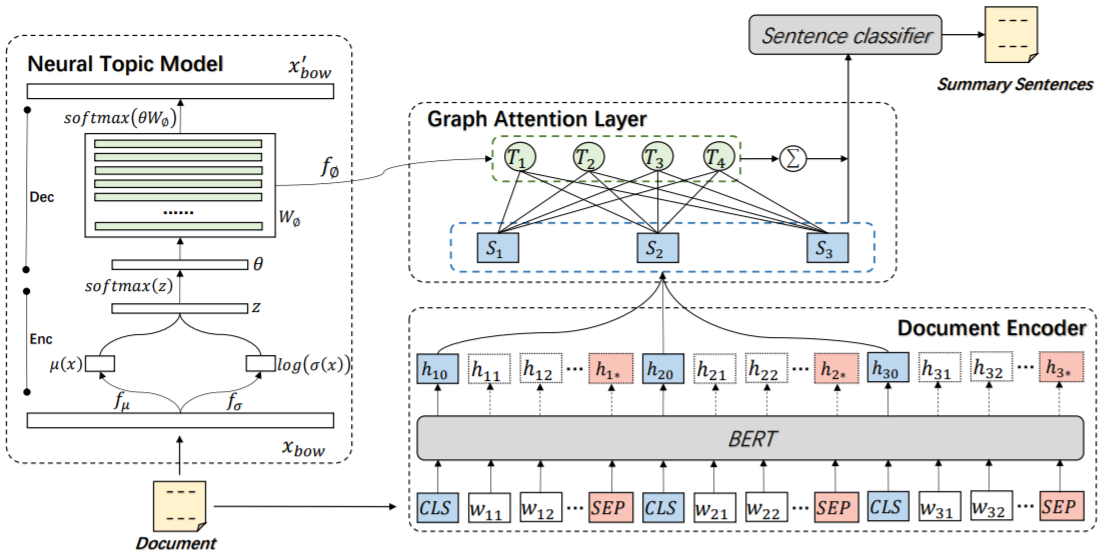
\includegraphics[width=.75\textwidth]{pics/Topic-GraphSum.PNG}
	\caption{Overview of Topic-GraphSum}
	\label{fig:topic_grpah_sum}
\end{figure}

如Fig.\ref{fig:topic_grpah_sum}所示,Topic-GraphSum模型主要分为三个部分,NTM(Neural Topic Model)用于从文档中抽取话题,Document Encoder用于生成每个句子的一个表征,再用前两部生成的topics和句子构造一个Heterogeneous Graph,使用GAT对该异构图进行学习,再将每个句子的表征输入到Sentecnce Classifer中,输出每个句子是否在Summarization中。